\chapter{From the Wave Function to the Fluid: Circulation and Vortices}\label{ch03}
% ---- local macros (unique names: chapters are combined into one document) -------------------------------------------
\InputIfFileExists{figures/ch03_numbers.tex}{}{\PackageWarning{ch03}{figures/ch03_numbers.tex is missing}}
\newcommand{\cthreeNum}[1]{\ifcsname cthree@#1\endcsname\csname cthree@#1\endcsname\else\textbf{??#1??}\PackageWarning{ch03}{number #1 is undefined}\fi}
\newcommand{\cthreeCode}[1]{\path{#1}}
\newlength{\cthreeOldES}\setlength{\cthreeOldES}{\emergencystretch}\setlength{\emergencystretch}{2.5em}
\let\cthreeOldTopFrac\topfraction\let\cthreeOldTextFrac\textfraction\let\cthreeOldFloatFrac\floatpagefraction
\renewcommand{\topfraction}{0.9}\renewcommand{\textfraction}{0.1}\renewcommand{\floatpagefraction}{0.85}% large figures stay on text pages instead of forming float pages

\section{An observation: circulation comes in whole units}\label{ch03:obs}

In 1961 W.~F.~Vinen detected single quanta of circulation in superfluid $^4$He with a vibrating wire; the quantum had the size that had been anticipated, $h/m$, with $m$ the mass of a helium atom \cite{Vinen1961,Zieve2023}.
Eighteen years later Yarmchuk, Gordon and Packard recorded photographically the positions of the quantized vortex lines in rotating superfluid helium and observed stationary arrays \cite{Yarmchuk1979}.
What these experiments measure is a number that no classical fluid has. The circulation $\Gamma=\oint\mathbf u\cdot\dd\mathbf l$ of the velocity around a closed curve drawn in the liquid takes only the values $0,\pm\kappa,\pm2\kappa,\dots$, where
\begin{equation}\label{ch03:eq-kappa}
  \kappa=\frac{h}{m}.
\end{equation}
The number is remarkable for what it does not contain. It is built from Planck's constant and the mass of one atom; no interaction strength, no density, no temperature enters. For $^4$He, with the exact SI value of $h$ and the atomic mass $m=\cthreeNum{mHeU}$~u (NIST), it is $\kappa=\cthreeNum{kappaHeFour}\times10^{-8}\ \mathrm{m^2/s}$ (computed in \texttt{figures/ch03\_compute.py}). In a vessel rotating at angular velocity $\Omega$ the quantized lines must on average imitate solid-body rotation, whose circulation per unit area is $2\Omega$; Feynman's counting \cite{Feynman1955} then gives an areal density $2\Omega/\kappa$ of lines, which is $\cthreeNum{feynmanDens}$ per cm$^2$ at $\Omega=1$~rad/s.

How can a complex wave function know about circulation? A wave function has a phase, and the velocity of the fluid it describes is the gradient of that phase. A gradient has no circulation, unless the phase cannot be defined everywhere, and a single-valued wave function can fail to define a phase only where it vanishes. A vortex is such a point. That is the chapter in three sentences; the pages that follow make each precise in the way of this book, as a statement a proof assistant has checked, as a computation the solver has run and, where an experiment exists, as a number to compare with it.

\begin{keybox}[What the chapter establishes]
\begin{enumerate}
\item \textbf{Circulation is quantized:} around a closed loop it is $w\kappa$ with $w$ an integer; sampled, this is a theorem about sums of principal phase differences (Lean, \cref{ch03:circ}).
\item \textbf{A vortex is a zero of $\psi$ with a winding number}, which the detector of every simulation code finds once the sampling resolves the phase (Lean, \cref{ch03:circ}); the solver shows how fine that is (\cref{ch03:counting}).
\item \textbf{Vortices are carried by the flow of the others:} a pair of separation $d$ moves at $\hbar/(md)$ in the plane; in a periodic box the integers that wind the phase around the torus add a uniform flow, $\cthreeNum{ubarOverV}\%$ of that speed at $d\approx12\xi$. The solver reproduces the corrected speed to about a percent for $d\ge6\xi$ and follows two leapfrogging pairs against a point-vortex model integrated with CVODE (\cref{ch03:speed,ch03:leap}).
\end{enumerate}
\end{keybox}

\begin{godfrinbox}{the other kind of excitation}
The experiments of Henri Godfrin and his collaborators probe quantum fluids through their excitations: inelastic neutron scattering at the Institut Laue--Langevin measured the dispersion relation of the phonon--maxon--roton excitations of superfluid $^4$He (Phys.\ Rev.\ B \textbf{103}, 104516 (2021), spectrometer IN5) \cite{Godfrin2021} and the density waves of two-dimensional liquid $^3$He (Nature \textbf{483}, 576 (2012)) \cite{Godfrin2012}.
In the linear theory such excitations are small oscillations about the uniform state, with a velocity that is the gradient of a single-valued phase: irrotational, without circulation. The vortices of this chapter are the other kind of excitation, states whose phase is \emph{not} single valued around a loop, which no small-amplitude wave can create or remove. Both live in the same $\psi$. \Cref{ch05} treats the first kind; the superfluid transition of a two-dimensional $^4$He film, measured by Bishop and Reppy \cite{BishopReppy1978} and described by the unbinding of vortex--antivortex pairs \cite{KosterlitzThouless1973}, is where the two meet (\cref{ch06}). Nothing here claims that those experiments observed vortices.
\end{godfrinbox}

\section{The wave function as a fluid}\label{ch03:madelung}

The model of the superfluid used throughout the book is the Gross--Pitaevskii equation \cite{Gross1961,Pitaevskii1961},
\begin{equation}\label{ch03:eq-gp}
  \ii\hbar\,\partial_t\psi=-\frac{\hbar^2}{2m}\nabla^2\psi+g\,|\psi|^2\psi,
\end{equation}
with $g>0$ the strength of a contact repulsion. For a dilute Bose gas at zero temperature it is the equation of the condensate; for liquid helium it is a model with the right structure (a complex order parameter, a compressible fluid, quantized circulation) and not the right numbers, since the core of a vortex in the liquid is of atomic size. The uniform state of density $n_0$ has two natural scales: the healing length $\xi=\hbar/\sqrt{mgn_0}$ and the speed of sound $c=\sqrt{gn_0/m}$. In the units $\hbar=m=g=n_0=1$ used by the solver both are $1$, so is the unit of time $\xi/c$, and the quantum of circulation is $\kappa=2\pi$.

Write the wave function in polar form, $\psi=\sqrt n\,\ee^{\ii S}$, with $n=|\psi|^2$ the density and $S$ the phase, and define the velocity
\begin{equation}\label{ch03:eq-u}
  \mathbf u=\frac{\hbar}{m}\nabla S .
\end{equation}
Substituting into \eqref{ch03:eq-gp} and separating the real and imaginary parts gives two real equations, found by Madelung in 1927 \cite{Madelung1927}:
\begin{align}
  \partial_t n+\nabla\!\cdot(n\,\mathbf u)&=0, \label{ch03:eq-cont}\\
  m\big(\partial_t\mathbf u+(\mathbf u\!\cdot\!\nabla)\mathbf u\big)&=-\nabla\big(g\,n+Q\big),\qquad Q=-\frac{\hbar^2}{2m}\,\frac{\nabla^2\sqrt n}{\sqrt n}. \label{ch03:eq-euler}
\end{align}
The first is conservation of mass. The second is Euler's equation for an inviscid compressible fluid of pressure $P=gn^2/2$, plus a \emph{quantum pressure} $Q$, which is all that remains of $\hbar$ once $\psi$ is written this way, and plus a constraint that no classical fluid obeys: $\mathbf u$ is a gradient, so $\nabla\times\mathbf u=0$ wherever $S$ is smooth. All the vorticity of a quantum fluid sits where $S$ is not smooth. The dictionary is short: density $n=|\psi|^2$, velocity $\mathbf u=(\hbar/m)\nabla S$, pressure $gn^2/2$, quantum pressure $Q$ (local, important only at scales $\lesssim\xi$), and vortex cores where $\psi=0$ and $S$ is undefined.

What the proof assistant says about it is limited and exact. The library does not contain \eqref{ch03:eq-cont} and \eqref{ch03:eq-euler}, which are textbook and derived above in two lines. What \texttt{MadelungSplit} proves is the algebra underneath: the squared gradient of $\psi=a\,\ee^{\ii S}$ splits into an amplitude part and a phase part, so the kinetic energy density of $\psi$ is the sum of the quantum-pressure term and the classical kinetic energy of the fluid.

\begin{leanbox}{MadelungSplit}
\begin{lstlisting}[style=lean,basicstyle=\ttfamily\footnotesize]
-- namespace QuantumFluids.Madelung
/-- **Kinetic-energy density split with physical constants.** With `rho = a^2` and superfluid
velocity components `u_i = (hbar/m) d_i S`, the kinetic energy density
`(hbar^2/2m) |grad psi|^2` equals the quantum-pressure term `(hbar^2/2m) |grad a|^2`
plus the hydrodynamic term `(m/2) rho |u|^2`. -/
theorem kinetic_density_split (ħ m a ga gS : ℝ) (hm : m ≠ 0) :
    ħ ^ 2 / (2 * m) * (ga ^ 2 + a ^ 2 * gS ^ 2)
      = ħ ^ 2 / (2 * m) * ga ^ 2 + m / 2 * a ^ 2 * (ħ / m * gS) ^ 2
\end{lstlisting}
\end{leanbox}

Here \texttt{ga} and \texttt{gS} stand for the components of $\nabla a$ and $\nabla S$ with $a=\sqrt n$. The statement of which this is the bookkeeping, \Lthm{MadelungSplit}{madelung_gradient_split}, is proved for an amplitude--phase wave function on $\mathbb R^n$ under the hypothesis that $a$ and $S$ are differentiable at the point; that hypothesis is genuine, and it is exactly what fails at a vortex core, where $a=0$ and $S$ is undefined. The module \texttt{MadelungNSE} restates the Madelung velocity in the vocabulary of a Lean formalisation of the Navier--Stokes problem statement and proves $\operatorname{div}\mathbf u=(\hbar/m)\Delta S$ there (\Lthm{MadelungNSE}{divergence_madelungVelocity}): bookkeeping, not a result about Navier--Stokes, which puts the two fluids in one formalism. That \eqref{ch03:eq-cont} and \eqref{ch03:eq-euler} look like the classical equations is an analogy; \cref{ch03:honest} says what the quantum fluid has that the classical one has not.

\section{Quantized circulation}\label{ch03:circ}

The circulation of the Madelung velocity \eqref{ch03:eq-u} around a closed curve $C$ on which $\psi\neq0$ is
\begin{equation}\label{ch03:eq-gamma}
  \Gamma(C)=\oint_C\mathbf u\cdot\dd\mathbf l=\frac{\hbar}{m}\oint_C\nabla S\cdot\dd\mathbf l=\frac{\hbar}{m}\,\Delta_C S ,
\end{equation}
that is, $\hbar/m$ times the change of the phase around $C$. The wave function must return to itself after one turn, so $S$ does so modulo $2\pi$: $\Delta_CS=2\pi w$ with $w$ an integer, and $\Gamma=w\,h/m=w\kappa$. This is the argument of Onsager \cite{Onsager1949} and Feynman \cite{Feynman1955}, and the integer $w$ is the \emph{winding number} of $\psi$ along $C$. It is topological: neither $g$ nor $n$ nor the dynamics enters, which is why the same quantum appears in a liquid and in a dilute gas.

Neither a simulation nor a photograph provides $S$ along a curve, only $\psi$ at points. The method of essentially every code that finds vortices, including this book's, is the following. Take points $\mathbf x_0,\dots,\mathbf x_n=\mathbf x_0$ along the loop, read the phases $\theta_i=\arg\psi(\mathbf x_i)$, replace each step $\theta_{i+1}-\theta_i$ by its principal value $\mathrm{pdiff}(\theta_i,\theta_{i+1})\in(-\pi,\pi]$, and add. Two questions arise. Is the sum a multiple of $2\pi$ whatever the sampling? And is the multiple the winding number of the continuous field? The library answers the first in \texttt{VortexWinding} and \texttt{QuantizedCirculation}, the second in \texttt{ContinuumWinding}.

\paragraph{Layer one: an identity of sums.} The principal difference differs from the true step by an integer multiple of $2\pi$ (\Lthm{VortexWinding}{pdiff_eq}), and on a closed loop the true steps telescope to $\theta_n-\theta_0=0$. Hence the sum of principal differences is an integer multiple of $2\pi$ (\Lthm{VortexWinding}{loop_sum_eq_mul}), and multiplying by $\hbar/m$ gives the following.

\begin{leanbox}{QuantizedCirculation}
\begin{lstlisting}[style=lean,basicstyle=\ttfamily\footnotesize]
-- namespace QuantumFluids.Circulation ; pdiff comes from QuantumFluids.VortexWinding
noncomputable def kappa (hbar m : ℝ) : ℝ := 2 * π * hbar / m

noncomputable def circulation (hbar m : ℝ) (S : ℕ → ℝ) (n : ℕ) : ℝ :=
  (hbar / m) * ∑ i ∈ Finset.range n, pdiff (S i) (S (i + 1))

/-- **Circulation is quantized.** Around any closed loop the circulation is an integer multiple of
the quantum `kappa`. -/
theorem circulation_quantized (hbar m : ℝ) (S : ℕ → ℝ) (n : ℕ) (hclosed : S n = S 0) :
    ∃ q : ℤ, circulation hbar m S n = (q : ℝ) * kappa hbar m := by
  obtain ⟨q, hq⟩ := loop_sum_eq_mul S n hclosed
  refine ⟨q, ?_⟩
  unfold circulation kappa
  rw [hq]
  ring
\end{lstlisting}
\end{leanbox}

The proof is the four lines shown; the content is in \Lthm{VortexWinding}{loop_sum_eq_mul}, whose proof is the telescoping argument just given (not shown). The same module proves \Lthm{QuantizedCirculation}{abs_circulation_ge}, that a nonzero circulation has magnitude at least $\kappa$ (no fraction of a quantum), and \Lthm{QuantizedCirculation}{circulation_quantum_attained}, that $\kappa$ itself is attained, by an explicit four-point loop whose last step wraps around by $2\pi$, the branch behaviour that \texttt{pdiff} exists to handle. The bound is therefore sharp. What neither theorem says is that the integer has anything to do with the field: for an arbitrary sequence of phases the sum is just as much a multiple of $2\pi$.

\paragraph{Layer two: the integer is the right one.} The next theorem closes that gap for a loop of field values.

\begin{leanbox}{ContinuumWinding}
\begin{lstlisting}[style=lean,basicstyle=\ttfamily\footnotesize]
-- namespace QuantumFluids.ContinuumWinding ; I = unit interval, [0,1]
/-- The `i`-th of `n` uniform sample points of the unit interval. -/
noncomputable def sample (n i : ℕ) : I := Set.projIcc 0 1 zero_le_one ((i : ℝ) / n)

/-- **The phase-winding vortex detector is correct.** For a continuous, nowhere-vanishing, closed loop
of field values, the sampled principal-branch loop sum of `arg` equals `2π` times the degree of the
loop, for every fine enough uniform sampling. -/
theorem detector_correct (c : C(I, ℂ)) (hne : ∀ t, c t ≠ 0) (hclosed : c 1 = c 0) :
    ∃ w : ℤ, ∃ n₀ : ℕ, 0 < n₀ ∧ ∀ n ≥ n₀,
      ∑ i ∈ Finset.range n, pdiff (Complex.arg (c (sample n i))) (Complex.arg (c (sample n (i + 1))))
        = (w : ℝ) * (2 * π)
\end{lstlisting}
\end{leanbox}

In words: if the loop $t\mapsto c(t)$ is continuous, closed and never zero, there are an integer $w$ (its degree) and a size $n_0$ such that every uniform sampling with $n\ge n_0$ points gives exactly $2\pi w$. The proof idea (abridged): the angle of $c$ is a closed loop on the circle $\mathbb R/2\pi\mathbb Z$; lift it to $\mathbb R$ along the covering map (Mathlib's path lifting); the lift is uniformly continuous on a compact interval (Heine--Cantor), so for large $n$ consecutive samples differ by less than $\pi$, every principal difference \emph{is} the true difference of the lift, the sum telescopes, and it equals the total change of the lift, $2\pi w$.

Two things the theorem does not give are what the solver supplies. It does not give $n_0$, which depends on how fast $c/|c|$ turns; the file says so. And its hypothesis \cthreeCode{hne} is where a vortex enters: on a loop through a zero of $\psi$ the lift, the degree and the theorem cease to exist. The failure mode of the standard algorithm is also a theorem: traversing an edge forth and back cancels exactly, except when the phase difference is exactly $\pi$, where both directions return $+\pi$ and add up to $2\pi$ (\Lthm{VortexWinding}{pdiff_add_rev_eq_two_pi_iff}); then two neighbouring plaquettes of a grid fail to cancel their shared edge and a spurious winding can appear. No true phase step between neighbouring samples may reach $\pi$.

\section{The vortex}\label{ch03:vortex}

\subsection{A vortex is a zero of \texorpdfstring{$\psi$}{psi}}\label{ch03:zero}Let a loop $C$ have winding $w\neq0$. If $\psi$ did not vanish anywhere on the disc bounded by $C$, shrinking $C$ continuously to a point would keep the winding an integer-valued continuous function, hence constant, and a point has winding zero. So $\psi$ vanishes somewhere inside. This is standard topology and it is \emph{not} in the library: the pinned Mathlib has no argument principle for general continuous maps, as the module \texttt{ContinuumWinding} says. What the library has is the discrete substitute of \cref{ch03:scale} below.

\subsection{Structure of one vortex}Around a singly quantized vortex at the origin the phase is the azimuth, $S=\theta$, so $\mathbf u=\hbar/(mr)\,\hat{\boldsymbol\theta}$ \emph{exactly}, whatever the density. The wave function is $\psi=\sqrt{n_0}\,f(r)\,\ee^{\ii\theta}$ where, in units of $\xi$,
\begin{equation}\label{ch03:eq-profile}
  f''+\frac{f'}{r}-\frac{f}{r^2}+2f(1-f^2)=0,\qquad f(0)=0,\quad f(\infty)=1 .
\end{equation}
A boundary-value solution (\texttt{figures/ch03\_gpvortex.py}) gives $f\simeq\cthreeNum{fSlope}\,r/\xi$ near the axis and $n=n_0f^2\simeq n_0\,(1-\xi^2/2r^2)$ far from it. The velocity decays like $1/r$ and the density disturbance like $1/r^2$: the flow of a vortex is long ranged, its core short ranged. By the split of the previous section the energy inside a disc of radius $R\gg\xi$ about the core then has a flow part $\int\frac12mn_0u^2\,\dd^2x=\pi(\hbar^2n_0/m)\ln(R/\xi)+\text{const.}$, which grows without bound with $R$, and a quantum-pressure part confined to the core. A single vortex therefore has an energy that depends on the size of the system.

\subsection{A pair, and the reduced model}\label{ch03:pair}A vortex--antivortex pair of separation $d$ has no net circulation, so the logarithm is cut off at $d$:
\begin{equation}\label{ch03:eq-pairE}
  E=2\pi\frac{\hbar^2n_0}{m}\ln\frac d\xi+2E_c ,
\end{equation}
with $E_c$ the energy of a core. Its momentum, the Kelvin impulse of the pair, is $P=mn_0\kappa d=2\pi\hbar n_0d$. Hamilton's equations for a localized object then give its speed by one line.

\begin{keybox}[The pair moves at $\hbar/(md)$]
Eliminating $d$ between $E=2\pi(\hbar^2n_0/m)\ln(d/\xi)+2E_c$ and $P=2\pi\hbar n_0d$ gives $E(P)=2\pi(\hbar^2n_0/m)\ln\!\big(P/2\pi\hbar n_0\xi\big)+2E_c$, and the speed of the pair is
\[
  U=\frac{\mathrm dE}{\mathrm dP}=\frac{2\pi\hbar^2n_0/m}{2\pi\hbar n_0d}=\frac{\hbar}{md}=\frac{\kappa}{2\pi d}.
\]
Helmholtz's picture gives the same answer: each vortex is carried by the velocity that the other induces at its position \cite{Helmholtz1858}, $\kappa/2\pi d$, perpendicular to the line joining them.
\end{keybox}

The second derivation has a Lean statement. The point-vortex law, in which a vortex of circulation $\Gamma$ at $w$ induces the velocity $\ii\Gamma/(2\pi\,\overline{(z-w)})$ at $z$ (complex notation), is textbook and was not in the library, so a small module was written for this chapter, \texttt{Ch03\_PointVortexPair.lean} (new in this book, not part of the \texttt{QuantumFluids} library), which proves what the law implies for a pair.

\begin{leanbox}{Ch03\_PointVortexPair \ (new)}
\begin{lstlisting}[style=lean,basicstyle=\ttfamily\footnotesize]
-- namespace QuantumFluids.Ch03PointVortexPair
/-- Velocity, as the complex number `u + i v`, induced at `z` by a point vortex of circulation `Γ` at `w`. -/
noncomputable def induced (Γ : ℝ) (z w : ℂ) : ℂ :=
  Complex.I * (Γ : ℂ) / (2 * (Real.pi : ℂ) * (starRingEnd ℂ) (z - w))

/-- **Speed of a pair carrying one quantum of circulation**: with `Γ = κ = 2πħ/m` the speed is `ħ / (m d)`. -/
theorem pair_speed_quantum (ħ m : ℝ) (hħ : 0 < ħ) (hm : 0 < m) {z w : ℂ} (h : z ≠ w) :
    ‖induced (2 * Real.pi * ħ / m) z w‖ = ħ / (m * ‖z - w‖)
\end{lstlisting}
\end{leanbox}

Besides \Lthm{Ch03PointVortexPair}{pair_speed_quantum} the module proves three facts that make up the point-vortex law for a pair:
\begin{itemize}
\item \Lthm{Ch03PointVortexPair}{induced_mul_conj}: the induced velocity times $\overline{(z-w)}$ is exactly $\ii\Gamma/2\pi$, so the velocity is perpendicular to the line joining the two points and has modulus $|\Gamma|/2\pi|z-w|$;
\item \Lthm{Ch03PointVortexPair}{pair_velocities_equal}: a vortex of circulation $-\Gamma$ and one of circulation $+\Gamma$ induce the \emph{same} velocity on each other, so a pair translates rigidly;
\item \Lthm{Ch03PointVortexPair}{separation_const}: along any differentiable motion obeying the two induced-velocity equations the separation is constant.
\end{itemize}
Nothing in the module concerns the Gross--Pitaevskii equation, the periodic box or more than two vortices; whether the Gross--Pitaevskii vortex obeys the law is what the solver is asked in \cref{ch03:solver}. The module compiles with zero errors and uses only the standard axioms (\cref{ch03:honest}). A real pair is not made of point vortices anyway: it is a solitary wave of the compressible field \cite{JonesRoberts1982}, whose speed departs from $\hbar/(md)$ at small $d$, by a correction that the programme's friction study puts at order $(\xi/d)^2$ \cite{Callens2026a}; \cref{ch03:speed} measures where it starts to matter.

\subsection{What a loop sees: scale-resolved winding}\label{ch03:scale}A loop of radius $R$ around one member of the pair sees winding $\pm1$; a loop that encloses both sees $0$. The winding as a function of the scale of the loop is a step at $R=d$, and a dipole is invisible from far away. The library proves this for any region of a grid, in the discrete form in which a code computes it: a region is a finite family of plaquettes, each with four corner phases, whose interior edges come in reversed pairs. If the charges of the plaquettes sum to zero the winding along the boundary is zero whatever the size of the region; if exactly one plaquette is charged, the boundary winding is its charge at every scale.

\begin{leanbox}{ScaleResolvedWinding}
\begin{lstlisting}[style=lean,basicstyle=\ttfamily\footnotesize]
-- namespace QuantumFluids.ScaleResolvedWinding ;  variable {m : ℕ} (Rg : Region m)
/-- **A dipole is invisible from outside.** If the charges inside sum to zero, the boundary winding
is zero, whatever the size of the region. -/
theorem dipole_invisible (hcut : ∀ e ∈ Rg.interior, Rg.step e ≠ π) (q : Fin m → ℤ)
    (hq : ∀ p, Rg.winding p = (q p : ℝ) * (2 * π)) (hneutral : ∑ p, q p = 0) :
    Rg.boundarySum = 0
\end{lstlisting}
\end{leanbox}

The hypothesis \cthreeCode{hcut} is again the branch-point condition: no interior edge may carry a phase step of exactly $\pi$. The proof is a discrete Stokes theorem: the boundary sum equals the sum of the plaquette loop sums (\Lthm{ScaleResolvedWinding}{stokes}), because every interior edge is traversed once in each direction.

\section{The solver: vortices in the projected Gross--Pitaevskii field}\label{ch03:solver}

\subsection{The engine and the imprint}\label{ch03:engine}

The engine is \texttt{qf-pgpe}, the Rust quantum-fluids crate of the rusty-SUNDIALS workspace, called through its Python extension \texttt{qf\_pgpe} (\cref{ch02}). It integrates the projected Gross--Pitaevskii equation $\ii\,\partial_t\psi=\mathcal P\big[-\tfrac12\nabla^2\psi+|\psi|^2\psi\big]$ \cite{Davis2001,Blakie2008} in the units of \cref{ch03:madelung} on a periodic square of side $L=64\,\xi$ with $128\times128$ grid points ($\Delta x=0.5\,\xi$). The projector $\mathcal P$ keeps the $3209$ Fourier modes with $|\mathbf k|\le k_{\rm cut}=\pi/\xi$, so the field is a band-limited function that can be evaluated at any point from its mode sum. The integrator is the integrating-factor Runge--Kutta scheme of order four with $\Delta t=0.01$. Vortices are placed by the engine's \cthreeCode{imprint_v2}: a product of Jacobi $\vartheta_1$ functions makes the phase periodic on the torus, the density is the Bernoulli profile of the imprinted flow, and the phase jump that a pair would otherwise leave across the box edge is removed by a uniform counterflow (the origin of \cref{ch03:speed}). They are found by \cthreeCode{detect}: the principal-difference winding of every grid plaquette, then a sub-grid refinement of the position, the detector that \texttt{ContinuumWinding} is about.

\begin{rustbox}{a vortex pair in \texttt{qf\_pgpe}}
\begin{lstlisting}[style=py,basicstyle=\ttfamily\footnotesize]
import numpy as np, qf_pgpe
s = qf_pgpe.Pgpe(128, 64.0)                  # n, L ; g = 1, dt = 0.01, k_cut = pi
pos0 = np.array([[26.13, 30.71], [38.13, 30.71]]); q = np.array([1, -1])   # separation 12, + on the left
c = s.imprint_v2(s.uniform(), pos0, q)       # periodic theta-function phase, Bernoulli density
for k in range(41):                          # t = 0, 1, ..., 40
    if k > 0:
        c = s.run(c, 1.0)                    # 100 IF-RK4 steps inside one Rust call
    dp, dq = s.detect(c)                     # plaquette windings -> sub-grid positions and charges
    E, N, P = s.energy(c), s.norm(c), s.momentum(c)
\end{lstlisting}
\smallskip\footnotesize
Condensed from \texttt{figures/ch03\_run.py}, which also tracks each vortex between snapshots. Output of the run used below (positions of the $+$ and $-$ vortex, energy $E$, norm $N$, momentum $P_y$):
\begin{lstlisting}[style=plainmono,basicstyle=\ttfamily\footnotesize]
t= 0  +(26.16, 30.72)  -(38.13, 30.72)  E=2069.120127  N=4096.000000  Py=72.9991
t=20  +(26.22, 32.58)  -(38.04, 32.58)  E=2069.120127  N=4096.000000  Py=72.9991
t=40  +(26.25, 34.46)  -(38.02, 34.47)  E=2069.120127  N=4096.000000  Py=72.9991
\end{lstlisting}
\end{rustbox}

Energy, norm and momentum are constants of the motion of the projected equation, and the run bears this out: over $40$ time units $E$ changes by a relative $\cthreeNum{energyDrift}$, $N$ by $\cthreeNum{normDrift}$ and $P_y$ by $\cthreeNum{momDrift}$. All timings in this chapter come from a shared eight-core machine whose load average was between $\cthreeNum{runLoadLo}$ and $\cthreeNum{runLoadHi}$ when the solver runs started; they are not benchmarks. A run of 40 time units took $\cthreeNum{runWallLo}$ to $\cthreeNum{runWallHi}$~s on it.

\subsection{Seeing the fluid in \texorpdfstring{$\psi$}{psi}}\label{ch03:see}

\Cref{ch03:fig-phasefield} shows one snapshot of the pair at $t=20$: the same complex array $\psi$ read as a phase, as a density and as a velocity. The cores are the dark dots of panel (a); around each of them the phase runs through all its values once, in opposite senses for the two; the streamlines of $\mathbf u=\operatorname{Im}(\bar\psi\nabla\psi)/|\psi|^2$ circle each core and join, between the vortices, into the jet that carries the pair upward.

\begin{figure}[tbp]\centering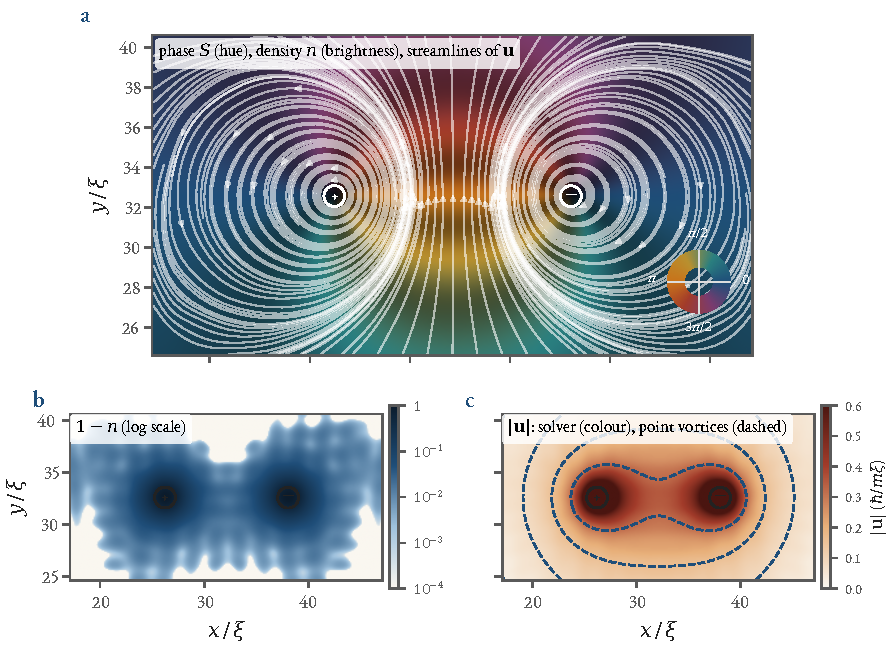
\includegraphics[width=\linewidth]{figures/ch03_phasefield.pdf}
\caption[One wave function, three faces]{One wave function, three faces (qf-pgpe, $t=20$, pair of separation $d\approx12\,\xi$, $+$ vortex on the left). \textbf{(a)}~Phase of $\psi$ (hue; global phase $\ee^{-\ii t}$ removed), density (brightness), streamlines of the Madelung velocity (white). \textbf{(b)}~Density deficit $1-n$, logarithmic; the faint rings are radiated sound. \textbf{(c)}~Speed $|\mathbf u|$: solver (colour) and periodic point vortices with their uniform flow (dashed contours at $0.04,0.08,0.16,0.32$).}
\label{ch03:fig-phasefield}\end{figure}

Three checks make the reading quantitative. First, the grid-level detector finds exactly $\cthreeNum{nPlus}$ plaquette of charge $+1$, $\cthreeNum{nMinus}$ of charge $-1$ and $\cthreeNum{nOther}$ of any other charge, and the same on a grid refined four-fold by spectral interpolation. The positions it reports are within $\cthreeNum{zeroOffset}\,\xi$ of exact zeros of the band-limited field: minimizing $|\psi|^2$ from the detected position finds points where $|\psi|^2\le\cthreeNum{zeroPsiMax}$, so the cores are zeros of $\psi$, as \cref{ch03:zero} requires. The largest principal phase step over all grid edges is $\cthreeNum{maxStepOverPi}\,\pi$ ($\cthreeNum{maxStepRefined}\,\pi$ on the refined grid), so no edge is near the branch point of \cref{ch03:circ}.

Second, panel (c): the relative rms difference between the Madelung velocity of the solver and the periodic point-vortex velocity (with the uniform flow of \cref{ch03:speed}) is $\cthreeNum{velRelInner}\%$ in the shell $1.5$--$3\,\xi$ about the cores and $\cthreeNum{velRelThreeSix}\%$ in the shell $3$--$6\,\xi$; without the uniform flow the second number is $\cthreeNum{velRelThreeSixNoSector}\%$. The phase of one Gross--Pitaevskii vortex is the azimuth exactly, which is why the point-vortex law holds so close to the core; I did not isolate the origin of the remaining two percent. Farther out the difference is $\cthreeNum{velFarRms}$ rms beyond $6\,\xi$, against a point-vortex speed of only $\cthreeNum{velFarPV}$, and it is not vortex flow: $\cthreeNum{curlFree}\%$ of its energy is curl-free and its rms equals that of the density ripple, $\cthreeNum{rmsDn}$ (the sound speed is $1$). It is the sound radiated while the imprinted state relaxes, visible as rings in panel (b) and absent from the point-vortex model.

Third, the first Madelung equation \eqref{ch03:eq-cont}. Evaluating $\partial_tn$ and $\nabla\!\cdot(n\mathbf u)$ with the engine's own right-hand side (no time stepping, no tracking), the continuity equation holds to a relative rms residual of $\cthreeNum{contRel}\%$ of $|\partial_tn|$ outside $3\,\xi$ from the cores. The residual is not noise: for the \emph{projected} equation it equals $-2\operatorname{Im}\big(\bar\psi\,(1-\mathcal P)[|\psi|^2\psi]\big)$, the part of the cubic term that the projector removes, an identity the script checks to $\cthreeNum{projIdentity}$ (largest residual $\cthreeNum{projResidualMax}$). The engine conserves the total norm, not the local continuity equation.

\subsection{Counting quanta}\label{ch03:counting}

Now the quantization of \cref{ch03:circ} on the solver field. Around the $+$ vortex, at its detected position, take circles of radius $R$ from $0.15\,\xi$ to $\cthreeNum{circRmax}\,\xi$ ($\cthreeNum{circLoops}$ loops), evaluate $\psi$ and $\nabla\psi$ at $1600$ points of each circle from the exact mode sum (not the grid), and compute the two quantities that the theory ties together: the circulation integral $\Gamma/\kappa$ with the Madelung velocity, and the winding found by the sum of principal differences of $\arg\psi$.

\begin{rustbox}{two ways to count the quanta}
\lstinputlisting[style=py,basicstyle=\ttfamily\footnotesize,linerange={24-24,26-27}]{figures/ch03_lib.py}
\medskip
\lstinputlisting[style=py,basicstyle=\ttfamily\footnotesize,linerange={48-48,51-53}]{figures/ch03_lib.py}
\medskip
\lstinputlisting[style=py,basicstyle=\ttfamily\footnotesize,linerange={55-55,58-62}]{figures/ch03_lib.py}
\smallskip\footnotesize
Docstrings omitted. \cthreeCode{pdiff} is the numpy form of \Lthm{VortexWinding}{pdiff}; \cthreeCode{ev} evaluates the band-limited field and its gradient at any point from the mode sum.
\end{rustbox}

\begin{figure}[tbp]\centering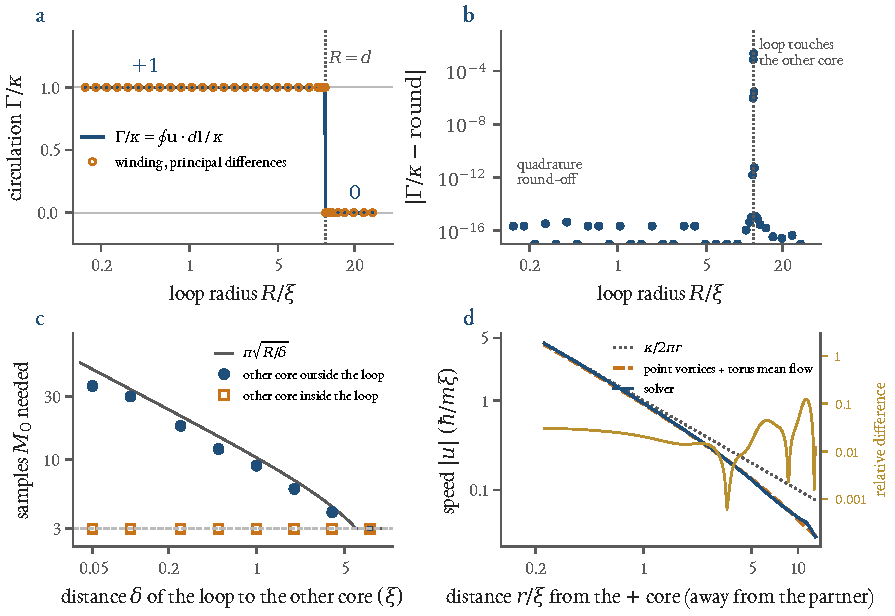
\includegraphics[width=\linewidth]{figures/ch03_circulation.pdf}
\caption[Counting quanta on the solver field]{Counting quanta on the solver field ($d\approx12\,\xi$, $t=20$, circles about the $+$ vortex). \textbf{(a)}~Circulation $\Gamma/\kappa$ (line) and detector winding (circles) against loop radius. \textbf{(b)}~Distance of $\Gamma/\kappa$ from the nearest integer. \textbf{(c)}~Smallest number of samples $M_0$ from which the principal-difference sum is right for every finer sampling, for a loop at distance $\delta$ from the other core, outside (blue) or inside (orange) the loop; worst of six starting angles. \textbf{(d)}~Speed along the line through both cores, on the side of the $+$ vortex away from its partner, against the distance $r$ to the core: solver, periodic point vortices, and $\kappa/2\pi r$ (dotted); gold, right axis: relative difference of the first two.}
\label{ch03:fig-circ}\end{figure}

The result, \cref{ch03:fig-circ}(a,b), is as sharp as the theorem allows. For every loop that encloses only the $+$ vortex ($R$ from $\cthreeNum{circRlo}$ to $\cthreeNum{circRhi}\,\xi$) $\Gamma/\kappa=1$ to within $\cthreeNum{circInnerDev}$; for every loop that encloses both ($R>d+1.4\,\xi$) it is zero to within $\cthreeNum{circOuterDev}$. The circulation of the solver is quantized in units of $\kappa$ to the accuracy of the quadrature, and the pair is invisible from outside, as \Lthm{ScaleResolvedWinding}{dipole_invisible} says it must be. The step from $1$ to $0$ takes place across the other core, where what limits the numbers is the quadrature and not the quantization: within $0.2\,\xi$ of that core the integrand is sharply peaked and $1600$ points no longer resolve it ($|\Gamma/\kappa-\text{integer}|=\cthreeNum{devDelta02}$, $\cthreeNum{devDelta01}$ and $\cthreeNum{devDelta005}$ at distances $0.2$, $0.1$ and $0.05\,\xi$). The detector, which only compares phases at consecutive samples, returns the right integer on all $\cthreeNum{circLoops}$ loops, including those three.

Panel (c) answers the question that \Lthm{ContinuumWinding}{detector_correct} leaves open: how large is $n_0$? Sample a circle with $M$ equally spaced points, for every divisor $M$ of $\cthreeNum{n0Mmax}$ and from one of six generic starting angles, and ask for the smallest $M_0$ from which every finer sampling gives the right winding; the worst of the six angles is plotted. A bare vortex needs $M_0=3$, since its step $2\pi/M$ must stay below $\pi$. If the other core lies \emph{inside} the loop, $M_0$ stays at $\cthreeNum{n0InMax}$ at every distance tested, down to $\delta=\cthreeNum{n0DeltaNear}\,\xi$. If it lies \emph{outside}, $M_0$ grows as the loop approaches it, from $\cthreeNum{n0OutFar}$ at $\delta=\cthreeNum{n0DeltaFar}\,\xi$ to $\cthreeNum{n0OutNear}$ at $\delta=\cthreeNum{n0DeltaNear}\,\xi$, as $\delta^{\cthreeNum{n0OutExp}}$. The reading is the hypothesis of the Lean theorems in quantitative form: the detector goes wrong exactly when the \emph{true} phase change between neighbouring samples reaches $\pi$. Along an arc of length $\ell=2\pi R/M$ passing a zero at distance $\delta$, the phase of that zero changes by up to $\pi-4\delta/\ell$, adding to the loop's own step $2\pi/M$ if the zero has the opposite charge and lies outside the loop, and subtracting from it if the zero lies inside. The sum reaches $\pi$ once $M\lesssim\pi\sqrt{R/\delta}$, and the measured $M_0$ are $\cthreeNum{n0RatioLo}$ to $\cthreeNum{n0RatioHi}$ times that. This derivation is mine, checked against these numbers, and is not in the library. So $n_0$ is finite, as the theorem says, but not a number the theorem could know: it depends on the distance to the nearest zero of $\psi$ and on whether that zero helps or opposes the winding being measured.

\paragraph{The torus has its own windings.} A loop does not have to be contractible. On the periodic grid the sums of principal differences along each of the $128$ rows and $128$ columns are again integers (to $\cthreeNum{torusDev}$), by the same theorem: all row windings are $0$, and the column windings are $1$ for the $\cthreeNum{nColsNonzero}$ columns between the two vortices and $0$ elsewhere. The integer pair measured outside that strip is the \emph{sector} of the state. The circulation of $\mathbf u$ around a cycle of the torus is $2\pi$ times it, so the \emph{mean} velocity over the box is fixed by the sector and the vortex positions, not by dynamics. For this pair the column windings give $\langle u_y\rangle=2\pi\,(\cthreeNum{nColsNonzero}\times0.5\,\xi)/L^2=\cthreeNum{ubarWinding}$, the integral of the Madelung velocity over the grid gives $\cthreeNum{ubarBox}$, and the position formula of \cref{ch03:speed} gives $\cthreeNum{ubarFormula}$; they agree to the width of one grid column. This small uniform flow has a large effect.

\subsection{Where the energy sits}\label{ch03:energy}

The identity of \Lthm{MadelungSplit}{kinetic_density_split} can be evaluated on the field: split $\frac12|\nabla\psi|^2$ at every point into $\frac12|\nabla\sqrt n|^2$ and $\frac12n|\mathbf u|^2$, on the refined $512^2$ grid, and integrate. The pointwise difference between the kinetic density and the sum of the two parts is $\cthreeNum{pointwiseErr}$ of its maximum (on the solver grid itself, $\cthreeNum{pointwiseErrCoarse}$): an algebraic identity holding to rounding error, not a measurement. What is measured is the partition. The integral of $\frac12|\nabla\psi|^2$ is $\cthreeNum{eKin}$ in units of $\hbar^2n_0/m$ (the Parseval sum of the Fourier amplitudes gives $\cthreeNum{eKinParseval}$); of this, $\cthreeNum{eFlow}$ ($\cthreeNum{fracFlow}\%$) is flow and $\cthreeNum{eQ}$ ($\cthreeNum{fracQ}\%$) is quantum pressure. The total energy of the pair above the uniform state is $\cthreeNum{eExcess}$; the remainder, $\frac12\int(n-1)^2\,\dd^2x$, is the interaction energy of the density disturbance.

\begin{figure}[tbp]\centering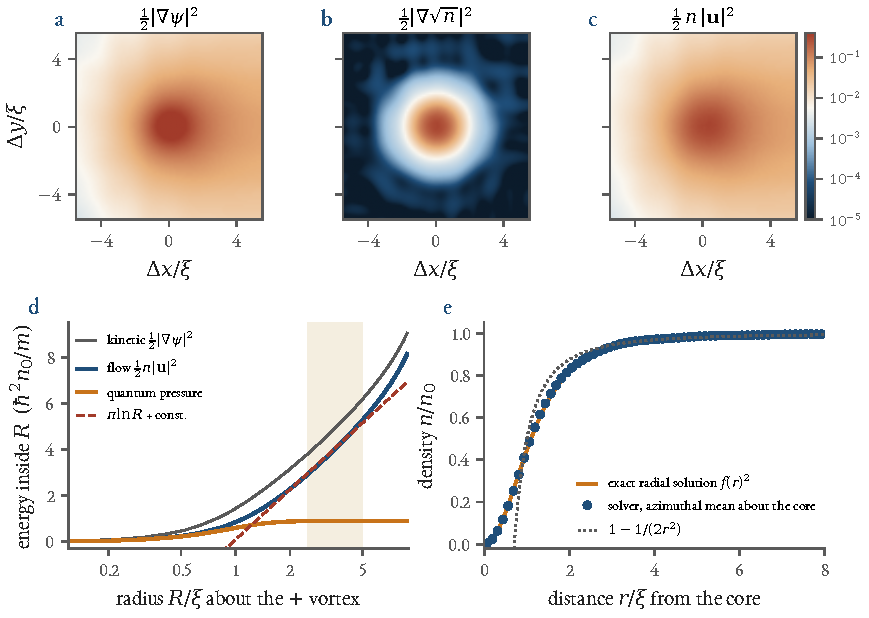
\includegraphics[width=\linewidth]{figures/ch03_energy.pdf}
\caption[Where the energy of a vortex sits]{Where the energy of a vortex sits ($d\approx12\,\xi$, $t=20$, refined grid). \textbf{(a--c)}~Kinetic, quantum-pressure and flow energy density near the $+$ vortex, one logarithmic scale. \textbf{(d)}~Energy inside radius $R$ about the core: the flow part follows $\pi\ln R$ in the shaded window and keeps growing, the quantum-pressure part saturates inside $3\,\xi$. \textbf{(e)}~Azimuthal mean density against the exact radial solution of \eqref{ch03:eq-profile}.}
\label{ch03:fig-energy}\end{figure}

\Cref{ch03:fig-energy} shows where the two parts live. The quantum pressure is a ring around the core: inside $3\,\xi$ it holds $\cthreeNum{qWithinThree}$ and inside $6\,\xi$ $\cthreeNum{qWithinSix}$, so it has saturated, whereas the flow energy inside the same radii is $\cthreeNum{flowWithinThree}$ and $\cthreeNum{flowWithinSix}$ and keeps growing. Fitting the flow energy against $\ln R$ for $2.5\le R/\xi\le5$ gives a slope of $\cthreeNum{slopePlus}$ about the $+$ vortex and $\cthreeNum{slopeMinus}$ about the $-$ vortex. The vortex's own azimuthal flow $\hbar/(mr)$ contributes $\cthreeNum{slopeSelf}$, to be compared with $\pi\bar n=\cthreeNum{slopePredicted}$ for the measured mean density $\bar n=\cthreeNum{nbarR}$ on the circle $R=3.75\,\xi$; the partner's flow and the uniform flow inside the disc contribute $\cthreeNum{slopePartner}$, the cross term $\cthreeNum{slopeCross}$, and the three add up to the measured slope. Panel (e) puts the core against its exact profile: they differ by at most $\cthreeNum{profMaxDiff}$ in density over $r\le8\,\xi$ ($n(1\,\xi)=\cthreeNum{nAtR1Solver}$ against $\cthreeNum{nAtR1Exact}$). I did not isolate the origin of this one-percent difference.

\subsection{The speed of a pair, and the lesson of the periodic box}\label{ch03:speed}

The Lean module of \cref{ch03:pair} says that a point-vortex pair of separation $d$ moves at $\hbar/(md)$. Does the Gross--Pitaevskii pair in a periodic box of side $64\,\xi$ do so? The solver was run for six separations, $d=4,6,8,12,16,20\,\xi$ (40 time units each; $d=12\,\xi$ is the run of the previous figures); the speed is the slope of the position of the pair's centre over $10\le t\le40$, the first ten time units containing the relaxation of the imprint. Three predictions can be made, each with one more ingredient than the last.

\begin{enumerate}
\item \emph{The plane law}, $v=\hbar/(md)$.
\item \emph{Point vortices on the torus.} Each vortex is carried by the velocity of the other and of all its periodic images. In Fourier space the velocity of vortices of charges $q_j$ at $\mathbf x_j$ is $\hat{\mathbf u}(\mathbf k)=\ii\,(k_y,-k_x)\,\hat\rho(\mathbf k)/|\mathbf k|^2$ with $\hat\rho(\mathbf k)=(\kappa/L^2)\sum_jq_j\ee^{-\ii\mathbf k\cdot\mathbf x_j}$, and the term $\mathbf k=0$ is absent: this is the field with \emph{zero mean flow}. The programme's earlier code has the same field in closed form (the Weiss--McWilliams pair function); the two agree to $\cthreeNum{fourierDiff}$ on the test configuration of the box below.
\item \emph{Plus the uniform flow that the windings of the torus force.} With positions taken in $[0,L)$, the circulation of the zero-mean-flow field around the $x$-cycle just above the line $y=0$ is $-(\kappa/L)\sum_jq_jy_j$, and around the $y$-cycle just above $x=0$ it is $+(\kappa/L)\sum_jq_jx_j$, which are not integer multiples of $\kappa$. The wave function requires $2\pi$ times an integer, and the integers measured in \cref{ch03:counting} are zero, so a uniform flow must make up the difference:
\begin{equation}\label{ch03:eq-ubar}
  \bar{\mathbf u}=\frac{\kappa}{L^2}\Big(\sum_jq_jy_j,\;-\sum_jq_jx_j\Big).
\end{equation}
For a pair of separation $d$ it has magnitude $\kappa d/L^2$ and the direction of the pair's own motion; it is the impulse of the pair divided by $mn_0L^2$. In units of the plane speed it is $\bar u/(\hbar/md)=2\pi d^2/L^2$, that is $\cthreeNum{ubarOverV}\%$ at $d=12\,\xi$ and $\cthreeNum{ubarOverV20}\%$ at $d=20\,\xi$.
\end{enumerate}

\begin{rustbox}{the periodic point-vortex model}
\lstinputlisting[style=py,basicstyle=\ttfamily\footnotesize,firstline=29,lastline=31]{figures/ch03_pv.py}
\medskip
\lstinputlisting[style=py,basicstyle=\ttfamily\footnotesize,linerange={68-68,70-74}]{figures/ch03_pv.py}
\smallskip\footnotesize
\texttt{pv\_velocity} is the programme's zero-mean-flow field (\texttt{exploration/pgpe/transport\_estimators.py}); the Fourier-series version \cthreeCode{fourier_velocity} of \texttt{figures/ch03\_pv.py} agrees with it to $\cthreeNum{fourierDiff}$ on a test configuration ($+$ at $(26.30,30.70)$, $-$ at $(38.10,31.20)$; recorded in \texttt{ch03\_numbers.json}).
\end{rustbox}

\begin{figure}[tbp]\centering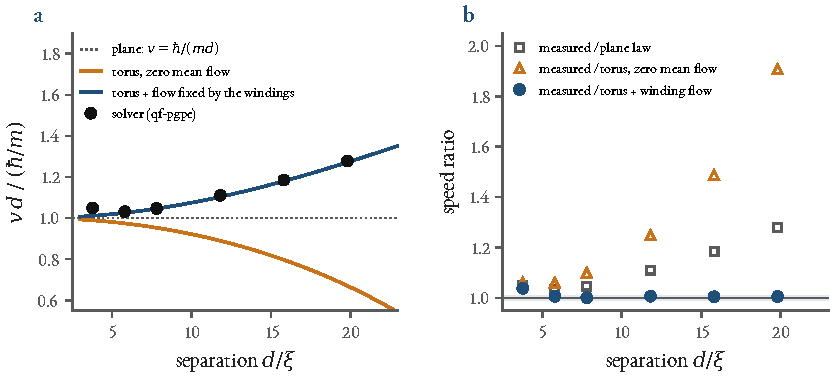
\includegraphics[width=\linewidth]{figures/ch03_pairspeed.pdf}
\caption[The speed of a vortex pair in the periodic box]{The speed of a vortex pair in the periodic box against its separation (six solver runs of 40 time units). \textbf{(a)}~$v\,d/(\hbar/m)$: the plane law ($=1$), point vortices on the torus with zero mean flow (orange), the same plus the uniform flow \eqref{ch03:eq-ubar} fixed by the windings (blue), and the measurements (black). \textbf{(b)}~Ratio of the measured speed to each prediction; the band is $\pm1\%$.}
\label{ch03:fig-speed}\end{figure}

\begin{table}[tbp]\centering\small
\begin{tabular}{@{}rccccccc@{}}
\toprule
$d/\xi$ & measured & plane & torus, & torus $+$ & \multicolumn{3}{c}{measured $/$}\\
 & & $1/d$ & zero flow & winding flow & plane & zero flow & $+$ flow\\
\midrule
3.8 & 0.2778 & 0.2648 & 0.2619 & 0.2677 & 1.049 & 1.061 & 1.038\\
5.8 & 0.1781 & 0.1726 & 0.1681 & 0.1770 & 1.032 & 1.059 & 1.006\\
7.8 & 0.1342 & 0.1282 & 0.1221 & 0.1341 & 1.047 & 1.099 & 1.001\\
11.8 & 0.0940 & 0.0847 & 0.0753 & 0.0934 & 1.110 & 1.249 & 1.006\\
15.8 & 0.0750 & 0.0633 & 0.0504 & 0.0746 & 1.185 & 1.488 & 1.005\\
19.8 & 0.0645 & 0.0505 & 0.0338 & 0.0642 & 1.278 & 1.908 & 1.005\\
\bottomrule
\end{tabular}

\caption{The measured speed of the pair against the three predictions (units $\hbar/m\xi$ per unit time; $d$ is the separation averaged over $10\le t\le40$; the predictions are evaluated at the tracked positions and averaged over the same window).}
\label{ch03:tab-speed}\end{table}

\Cref{ch03:fig-speed} and \cref{ch03:tab-speed} give the result. The measured speed exceeds the plane law by $\cthreeNum{pctPlaneMin}$ to $\cthreeNum{pctPlane8}\%$ for $d\le8\,\xi$ and by $\cthreeNum{pctPlane12}\%$, $\cthreeNum{pctPlane16}\%$ and $\cthreeNum{pctPlane20}\%$ at $d=12,16,20\,\xi$. The torus point-vortex speed with zero mean flow is too small, and increasingly so with $d$: the measured speed is $\cthreeNum{scanTwelveRatioPvz}$, $\cthreeNum{scanSixteenRatioPvz}$ and $\cthreeNum{scanTwentyRatioPvz}$ times it at $d=12,16,20\,\xi$, so the discrepancy is not a core effect, which would shrink with $d$. With the uniform flow \eqref{ch03:eq-ubar} the ratios are $\cthreeNum{scanSixRatioPv}$, $\cthreeNum{scanEightRatioPv}$, $\cthreeNum{scanTwelveRatioPv}$, $\cthreeNum{scanSixteenRatioPv}$ and $\cthreeNum{scanTwentyRatioPv}$ for $d\ge6\,\xi$: the prediction reproduces the solver to about one percent, with no fitted parameter. At $d\approx4\,\xi$ the measured speed is $\cthreeNum{pctPvFour}\%$ above it; there the pair is a solitary wave of the compressible field rather than two point vortices \cite{JonesRoberts1982}. That is the sign and size of the discrepancy, not a derivation of it.

The same effect appeared in the programme's study of friction on vortices, where it was first misread: the ratios of the box-frame speed to the zero-mean-flow prediction there ($1.06,1.06,1.10$ and $1.49$ at $d=4,6,8$ and $16\,\xi$, in its table of $T=0$ kinematics \cite{Callens2026a}; different runs and imprint position) are the numbers measured here. The lesson is general. A vortex pair carries impulse, and a periodic box has no infinity to which to assign it, so the fluid as a whole moves; the amount is a property not of the dynamics but of the integers that wind the phase around the torus, whose existence \Lthm{VortexWinding}{loop_sum_eq_mul} guarantees.

The field momentum is conserved ($P_y=\cthreeNum{momPy}$, relative change $\cthreeNum{momDrift}$) but is $\cthreeNum{momRatio}\%$ of the impulse $2\pi d=\cthreeNum{momImpulse}$ at $t=20$. The difference is the density deficit: the momentum is $\int n\,u_y\,\dd^2x$, and the integral of $u_y$ alone over the box, $L^2\times\cthreeNum{ubarBox}$, exceeds it by $\int(1-n)\,u_y\,\dd^2x$, which is $\cthreeNum{momDeficitPct}\%$ of it. The separation shrinks by $\cthreeNum{dipoleMomRelShrink}\%$ over the run, so the impulse of the vortices falls while the field momentum does not; the balance must be carried by the sound field.

\subsection{Leapfrogging pairs, and the reduced model in CVODE}\label{ch03:leap}

\begin{figure}[tbp]\centering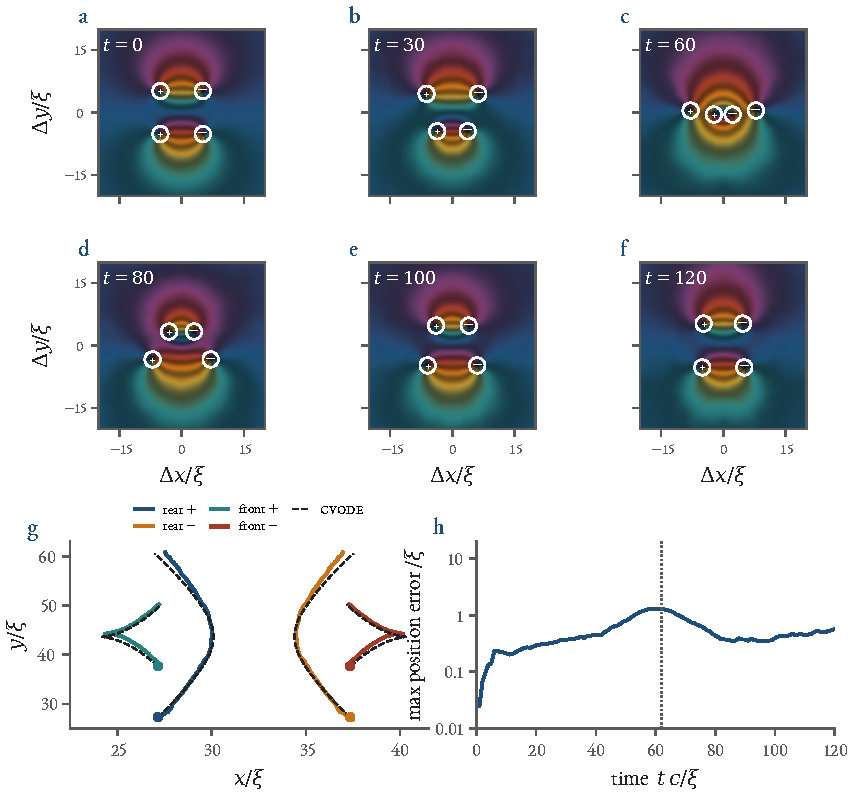
\includegraphics[width=\linewidth]{figures/ch03_leapfrog.pdf}
\caption[Two vortex pairs leapfrog]{Two vortex pairs leapfrog (qf-pgpe, $L=64\,\xi$, 120 time units). \textbf{(a--f)}~The wave function at six times (colour code of \cref{ch03:fig-phasefield}), the view re-centred on the four vortices. \textbf{(g)}~Tracked vortices (solid) and the periodic point-vortex model integrated with CVODE (dashed) from the detected positions at $t=0$ (dots). \textbf{(h)}~Largest distance between a tracked vortex and its model trajectory; dotted: the time at which the rear pair passes the front pair in the solver.}
\label{ch03:fig-leap}\end{figure}

Two pairs of the same sense, one behind the other, give a motion familiar from classical hydrodynamics as the leapfrogging of vortex rings. The rear pair is drawn forward by the flow of the front pair, narrows as it accelerates, passes through the front pair, which has widened and slowed, and then widens in its turn while the other narrows. The solver was started with four vortices $+,-,+,-$ at the corners of a square of side $10.3\,\xi$ and run for $\cthreeNum{quadT}$ time units; \cref{ch03:fig-leap} shows the wave function at six times and the tracked vortices.

The reduced model is the periodic point-vortex model of \cref{ch03:speed}: four vortices obeying $\dot{\mathbf x}_a=\mathbf u_a(\mathbf x)+\bar{\mathbf u}$, with $\mathbf u_a$ the zero-mean-flow field of the other three and their images and $\bar{\mathbf u}$ the uniform flow \eqref{ch03:eq-ubar}, constant here because $\sum_jq_j\mathbf x_j$ is conserved. It is integrated with CVODE from the positions detected at $t=0$.

\begin{rustbox}{CVODE integrates the point-vortex model}
\lstinputlisting[style=py,basicstyle=\ttfamily\footnotesize,firstline=83,lastline=85]{figures/ch03_pv.py}
\medskip
\lstinputlisting[style=py,basicstyle=\ttfamily\footnotesize,firstline=87,lastline=92]{figures/ch03_pv.py}
\smallskip\footnotesize
Excerpt of \cthreeCode{integrate_cvode} (\texttt{figures/ch03\_pv.py}; \texttt{rhs} advances the state, the loop restarts CVODE at each output time). Run with the rusty-SUNDIALS build of commit \texttt{5db8041}, \texttt{rusty\_sundials.\_\_file\_\_} recorded in \texttt{ch03\_numbers.json}. Result for the four-vortex run: \cthreeNum{cvodeCalls} right-hand-side calls in \cthreeNum{cvodeSeconds}~s for 120 time units on the loaded machine (the right-hand side is a Python function called through the binding); an independent integration of the same equations with SciPy's DOP853 at tolerance $10^{-12}$ differs from the CVODE trajectory by at most $\cthreeNum{cvodeVsDop}\,\xi$ over the whole run, and the dipole moment $\sum_jq_j\mathbf x_j$, conserved by the equations, is conserved by CVODE to $\cthreeNum{cvodeDipole}$.
\end{rustbox}

Against the solver the model does well, and one cause of the difference can be measured. The rear pair narrows from $\cthreeNum{quadWidth0}\,\xi$ to $\cthreeNum{quadRearMin}\,\xi$ in the solver ($\cthreeNum{quadRearMinODE}\,\xi$ in the model) and the front pair widens to $\cthreeNum{quadFrontMax}\,\xi$ ($\cthreeNum{quadFrontMaxODE}\,\xi$); the rear pair passes the front pair at $t=\cthreeNum{passGP}$ in the solver and at $t=\cthreeNum{passODE}$ in the model, $\cthreeNum{passDiff}$ time units ($\cthreeNum{passDiffPct}\%$) earlier; by $t=\cthreeNum{quadT}$ the roles are exchanged, the former rear pair being $\cthreeNum{quadYLead}\,\xi$ ahead in the solver. The largest distance between a tracked vortex and its model trajectory is $\cthreeNum{quadErr10}$, $\cthreeNum{quadErr20}$ and $\cthreeNum{quadErr40}\,\xi$ at $t=10,20,40$, rises to $\cthreeNum{quadErr60}\,\xi$ at the passage, where a small error in timing becomes a large error in position because the vortices move fastest, and is $\cthreeNum{quadErr100}$ and $\cthreeNum{quadErr120}\,\xi$ at $t=100,120$.

Where does the difference come from? Part of it is the imprint: the imprinted state relaxes, and the error is already $0.22\,\xi$ at $t=8$. Restarting the model from the tracked positions at a later time tests this (with DOP853, which takes seconds). Started at $t=0,10,20,40$ the model passes the front pair at $t=\cthreeNum{restartPass0},\cthreeNum{restartPass10},\cthreeNum{restartPass20},\cthreeNum{restartPass40}$ against $\cthreeNum{passGP}$ in the solver, and its largest error over the rest of the run is $\cthreeNum{restartErrMax0},\cthreeNum{restartErrMax10},\cthreeNum{restartErrMax20},\cthreeNum{restartErrMax40}\,\xi$; ten time units after a restart at $t=20$ it is $\cthreeNum{restartErrTen20}\,\xi$. So most of the passing-time discrepancy is the first twenty to forty time units of relaxation, not an inability of point vortices to leapfrog. What is left (a restart at $t=40$: $0.4\,\xi$ at worst, a passing time within $0.5$ time units) is what point vortices lack, the core structure and the compressibility of the field; I did not separate the two. The closest approach inside a pair is $\cthreeNum{quadMinSepGP}\,\xi$, where the speed excess of the previous subsection lies between $\cthreeNum{scanSixPctPv}\%$ and $\cthreeNum{pctPvFour}\%$. The impulse $\sum_jq_j\mathbf x_j$ is conserved exactly in the model and falls by $\cthreeNum{quadDipoleChange}\%$ over the run in the solver, while the total field momentum is conserved to $\cthreeNum{quadMomDrift}$ and the energy to $\cthreeNum{quadEnergyDrift}$.

\section{What this chapter establishes, and what it does not}\label{ch03:honest}

\begin{honestbox}
\textbf{Proved in Lean} (standard axioms \texttt{propext}, \texttt{Classical.choice}, \texttt{Quot.sound}: by the programme's compile audit for \texttt{VortexWinding}, \texttt{MadelungSplit} and \texttt{MadelungNSE}; re-compiled for this chapter for \texttt{QuantizedCirculation}, \texttt{ContinuumWinding} and \texttt{ScaleResolvedWinding}). Sums of principal phase differences around a closed loop are integer multiples of $2\pi$, so the discrete circulation is $q\kappa$, a nonzero one has $|\Gamma|\ge\kappa$, and $\kappa$ is attained; for a continuous nowhere-vanishing closed loop the detector returns $2\pi w$ for every fine enough sampling, $n_0$ unquantified; the kinetic energy density of $a\,\ee^{\ii S}$ splits into an amplitude and a phase term; $\operatorname{div}\mathbf u=(\hbar/m)\Delta S$ in a Navier--Stokes vocabulary; a dipole is invisible to the discrete winding of any enclosing region. \emph{New here} (\texttt{book/lean/Ch03\_PointVortexPair.lean}, zero errors, same three axioms): the point-vortex law implies that a $\pm\Gamma$ pair translates rigidly at $\hbar/(md)$ for $\Gamma=\kappa$, at constant separation.

\textbf{Not in Lean}, and textbook: the Madelung equations; the vortex profile \eqref{ch03:eq-profile}; the energy and impulse of a pair and $U=\mathrm dE/\mathrm dP$; that a Gross--Pitaevskii vortex moves with the velocity induced by the others; that a nonzero winding implies a zero of $\psi$ inside.

\textbf{Simulated} (qf-pgpe at $128^2$, $k_{\rm cut}=\pi/\xi$, zero temperature, one initial condition per case, up to $120$ time units; CVODE for the reduced model). Circulation is an integer to $\cthreeNum{circInnerDev}$ and the detector is right on all $\cthreeNum{circLoops}$ loops; $\cthreeNum{fracFlow}\%$ of the kinetic energy of the pair is flow; the pair speed equals the torus point-vortex prediction with the winding-fixed flow to about $1\%$ for $d\ge6\,\xi$ ($\cthreeNum{pctPvFour}\%$ above it at $d\approx4\,\xi$); the model follows the leapfrog to $\cthreeNum{quadErrMax}\,\xi$ at worst over $120$ time units, with a $\cthreeNum{passDiffPct}\%$ error in the passing time, mostly the relaxation of the imprint.

\textbf{Analogy only.} The Madelung equations have the form of those of a classical inviscid fluid, and vortex pairs in the quantum fluid move like pairs in the classical one. LL-15: what the two systems must share for this to transfer is a velocity that is a gradient away from a few singular points that the flow carries; the quantum fluid adds the single-valuedness of $\psi$ (quantized circulation, no continuous vorticity), the point-vortex model lacks the compressibility of the field. Nothing here is a prediction for the liquid helium of \cref{ch03:obs}: Gross--Pitaevskii is a model of it.

\textbf{What failed or was wrong on the way.} (i) The first compilation of the new Lean file failed on three proofs (a simplifier normal form for the conjugate of a difference, an unsolved imaginary part, the same form inside a norm); the version shown is the one that compiled. (ii) My first guess for the sampling threshold $n_0$ (the number of samples needed to resolve a $\pi$ step across the distance to the other core) was wrong twice over: loops started towards that core needed no extra samples, and with generic starting angles the threshold depends on whether the other zero is inside or outside the loop and grows as $\delta^{-1/2}$. (iii) In the programme's friction study the excess of the measured pair speed over the zero-mean-flow prediction (up to $49\%$) was first read as an imprint transient; it is the uniform flow of the torus (CLAIM-082 of the programme's ledger). (iv) The first CVODE run of the reduced model used a stale build of the Python module, older than the repair of commit \texttt{5db8041} of rusty-SUNDIALS: it needed $\cthreeNum{staleCalls}$ right-hand-side calls and differed from DOP853 by $\cthreeNum{staleVsDop}\,\xi$, against $\cthreeNum{cvodeCalls}$ calls and $\cthreeNum{cvodeVsDop}\,\xi$ for the repaired build, with which the run was redone.
\end{honestbox}

\section*{Exercises}\label{ch03:ex}
\addcontentsline{toc}{section}{Exercises}

\paragraph{Exercise 1.} \emph{Two samples are not enough.} A vortex has phase $\theta(\varphi)=\varphi$ along a circle centred on it. (a) For $n=2$ samples, at $\varphi=0$ and $\pi$, compute the sum of principal differences for the counter-clockwise and for the clockwise traversal. (b) Explain with \Lthm{VortexWinding}{pdiff_add_rev_eq_two_pi_iff} why both give the same answer, and why \Lthm{ContinuumWinding}{detector_correct} says nothing about this sampling. (c) For which $n$ is the sum right for every starting angle? \emph{Hint:} the principal value of a step of exactly $\pi$ is $+\pi$ in both directions; for (c) all steps $2\pi/n$ must be below $\pi$.

\paragraph{Exercise 2.} \emph{The mean flow of the torus.} (a) Show from \eqref{ch03:eq-ubar} that $\bar u/(\hbar/md)=2\pi d^2/L^2$ and evaluate it for $d=6,12,16\,\xi$, $L=64\,\xi$. (b) Derive \eqref{ch03:eq-ubar} for one pair, the $+$ vortex at $(x_1,y)$ and the $-$ vortex at $(x_2,y)$. \emph{Hint:} the circulation of the zero-mean-flow field around a row $y=\text{const}$ is piecewise constant in $y$ (it changes by $\mp\kappa$ across a vortex), has zero mean over $y$, and the wave function requires an integer multiple of $2\pi$. (c) In which direction, and how fast, does the pair with the $+$ vortex \emph{below} the $-$ vortex, at the same $x$, move? \emph{Hint:} the box has fourfold symmetry; check the direction with \cthreeCode{vortex_velocity}.

\paragraph{Exercise 3.} \emph{Run it.} With \texttt{qf\_pgpe}, imprint the pair of \cref{ch03:engine} with $d=12\,\xi$ in a box of side $L=96\,\xi$ with $192^2$ grid points (the same $\Delta x$), run for $40$ time units and measure the speed as in \cref{ch03:speed}. Predict it first from \eqref{ch03:eq-ubar} and the zero-mean-flow field (\cthreeCode{vortex_velocity} with \texttt{L=96}); what changes between the two boxes, and by how much? \emph{Hint:} the uniform flow scales as $L^{-2}$, and so, to leading order, does the correction from the images. For comparison, my run of this recipe (\cthreeNum{exWall}~s on the loaded machine) gave $v=\cthreeNum{exVmeas}$ against the prediction $\cthreeNum{exVpv}$, where the same pair in the $64\,\xi$ box moves at $\cthreeNum{scanTwelveMeas}$.

\section*{Notes and further reading}
\addcontentsline{toc}{section}{Notes and further reading}

The hydrodynamic form of the Schr\"odinger equation is Madelung's \cite{Madelung1927}; the quantization of circulation was proposed by Onsager \cite{Onsager1949} and applied by Feynman to rotating helium \cite{Feynman1955}. It was detected in single quanta in Vinen's vibrating-wire experiment \cite{Vinen1961} (Zieve's retrospective \cite{Zieve2023} is a good entry point) and the arrays of lines were photographed by Yarmchuk, Gordon and Packard \cite{Yarmchuk1979}. For the Gross--Pitaevskii vortex see \cite{Gross1961,Pitaevskii1961} and the books of Pitaevskii and Stringari \cite{PitaevskiiStringari2016} and, for the liquid, Donnelly \cite{Donnelly1991}; vortices are carried by the flow of the others in Helmholtz's analysis \cite{Helmholtz1858}, and the pair as a solitary wave of the compressible field is the subject of Jones and Roberts \cite{JonesRoberts1982}. The projected method is reviewed in \cite{Blakie2008}; the engine is \cite{Callens2026sw}, the library \cite{Callens2026lib}, and the friction study that identified the mean flow of the torus \cite{Callens2026a}. The pairs of this chapter are what unbinds in \cref{ch06}, what moves with dissipation in \cref{ch07}, and what a moving obstacle sheds in \cref{ch09}, in the simulations of Kwon and Shin \cite{KwonShin2026prr}.

\setlength{\emergencystretch}{\cthreeOldES}
\let\topfraction\cthreeOldTopFrac\let\textfraction\cthreeOldTextFrac\let\floatpagefraction\cthreeOldFloatFrac
